\documentclass{beamer}

\usepackage{preamble}

\begin{document}

\begin{frame}[plain]
  \begin{columns}
    \begin{column}{1.01\textwidth}
      \titlepage
    \end{column}
  \end{columns}
\end{frame}

% \frame[plain]{\titlepage}

\small
\setbeamercovered{transparent}

{
\setbeamertemplate{headline}[default]
\begin{frame}
\frametitle{\LARGE{Contenidos}}
\tableofcontents[pausesections]
\end{frame}
}

\section{Preliminares}

\subsection{Espacios \texorpdfstring{$L^p$}{Lp}}

\begin{frame}
    \begin{block}{}
        Si $1\leq p<\infty$, se define
        \[L^p(\T) = \Bigl\{f \colon \R \to \C \mid f \textup{ medible y } 2\pi\textup{-periódica,} \integral{-\pi}{\pi}{|f(t)|^p} < \infty \Bigr\},\]
        \[\|f\|_p = \left(\frac{1}{2\pi}\integral{-\pi}{\pi}{|f(t)|^p}\right)^{\frac{1}{p}}, \qquad f \in L^p(\T).\]
    \end{block}
    \pause
    \begin{block}{}
        Para $p = \infty$, se define
        \[L^\infty(\T) = \Bigl\{f \colon \R \to \C \mid f \textup{ medible y } 2\pi\textup{-periódica,} \supes_{x \in \R} |f(x)| < \infty\Bigr\},\]
        \[\|f\|_{\infty} = \supes_{x \in \R} |f(x)|, \qquad f \in L^\infty(\T).\]
    \end{block}
    \pause
    Identificamos funciones iguales en casi todo punto.
\end{frame}

\subsection{Series de Fourier}

\begin{frame}
    \begin{block}{}
        Sea $f \in L^1(\T)$.
        \begin{itemize}
            \item<1-> Se definen los \emph{coeficientes de Fourier de $f$} como
            \[c_k(f) = \frac{1}{2\pi}\integral{-\pi}{\pi}{f(t)e^{-ikt}}, \qquad k \in \Z.\]
            \item<2-> La \emph{serie de Fourier de $f$} es la serie formal
            \[Sf(x) = \sum_{ k \in \Z} c_k(f)e^{ikx}.\]
            \item<3-> La suma parcial $n$-ésima esta serie es
            \[S_nf(x) = \sum_{k =-n}^n c_k(f)e^{ikx}.\]
        \end{itemize}
    \end{block}
\end{frame}

\begin{frame}
    \begin{block}{}
        Un \emph{polinomio trigonométrico} es una función $F \colon \R\to\C$ de la forma
        \[F(x) = \sum_{k=-n}^n c_ke^{-ikx},\]
        con $n\in\N$ y $c_k\in\C$ para todo $k\in\Z$ con $|k|\leq n$.
    \end{block}
    \pause
    \begin{block}{}
        Dado $n \in \N \cup \{0\}$, el \emph{núcleo de Dirichlet de orden $n$} es la función $D_n \colon \R \to \C$ definida por
        \[D_n(x) = \sum_{k=-n}^n e^{ikx}.\]
        \pause
        Si $f \in L^1(\T)$, $n \in \N$ y $x \in \R$,
        \[S_nf(x) = f \ast D_n(x).\]
    \end{block}
\end{frame}

\begin{frame}
    \begin{figure}[H]
    \centering
    \begin{subfigure}[b]{0.49\textwidth}
        \centering
        \includegraphics[scale = 0.49]{plot1/main.pdf}
    \end{subfigure}
    \begin{subfigure}[b]{0.49\textwidth}
        \centering
        \includegraphics[scale = 0.49]{plot2/main.pdf}
    \end{subfigure}
    \par\bigskip
    \begin{subfigure}[b]{0.49\textwidth}
        \centering
        \includegraphics[scale = 0.49]{plot3/main.pdf}
    \end{subfigure}
    \begin{subfigure}[b]{0.49\textwidth}
        \centering
        \includegraphics[scale = 0.49]{plot4/main.pdf}
    \end{subfigure}
    \end{figure}
\end{frame}

\subsection{Resultados de Análisis Funcional}

\begin{frame}
    \begin{block}{}
        Si $T \colon X \to Y$ es lineal y continua, se define la \emph{norma de $T$} como
        \[\|T\| = \inf\{C > 0 \colon \|T(x)\|_Y \leq C\|x\|_X \textup{ para todo } x \in X\}.\]
        Se tiene que
        \[\|T\| = \sup_{x \neq 0} \frac{\|T(x)\|_Y}{\|x\|_X} = \sup_{\|x\|_X = 1} \|T(x)\|_Y = \sup_{\|x\|_X \leq 1} \|T(x)\|_Y.\]
    \end{block}
    \pause
    \begin{block}{Teorema de la acotación uniforme}
    Sea $\{T_j\}_{j \in I}$ una familia de aplicaciones lineales y continuas de $X$ en $Y$. Supongamos que
    \begin{itemize}
        \item $(X,\|\cdot\|_X)$ es de Banach.
        \item Para cada $x \in X$, el conjunto $\{T_j(x) \colon j \in I\}$ es acotado en $Y$.
    \end{itemize}
    Entonces el conjunto $\{\|T_j\| \colon j \in I\}$ es acotado en $\R$.
    \end{block}
\end{frame}

\section{Convergencia puntual}

\subsection{Una función continua cuya serie de Fourier diverge en un punto}

\begin{frame}
    \begin{block}{Teorema}
        Existe una función continua cuya serie de Fourier diverge en un punto.
    \end{block}
    \pause
    Consideramos la familia de aplicaciones lineales y continuas $\{T_n\}_{n\in\N}$, donde
    \begin{align*}
        T_n \colon \mathcal{C}([-\pi,\pi]) &\longrightarrow \R, \\
        g &\longmapsto S_ng(0).
    \end{align*} Se demuestra que
    \[\|T_n\| = \|D_n\|_1 \nconv \infty.\]
    Por el teorema de la acotación uniforme, existe $g \in \mathcal{C}([-\pi,\pi])$ con
    \[\sup_{n\in\N}|T_n(g)| = \infty.\]
\end{frame}

\subsection{Una función de \texorpdfstring{$L^1$}{L1} cuya serie de Fourier diverge en todo punto}

\begin{frame}
    \begin{block}{}
        Sea $\alpha \in \R$.
        \begin{itemize}
            \item Si $\alpha \geq 0$, se define la \emph{parte fraccionaria de $\alpha$} como $\angles{\alpha} = \alpha - E(\alpha)$.
            \item Si $\alpha < 0$, se define la \emph{parte fraccionaria de $\alpha$} como $\angles{\alpha} = \angles{-\alpha}$.
        \end{itemize} 
        \begin{figure}
        \centering
        \includegraphics[scale = 0.9]{images/1.pdf}
        \end{figure}
    \end{block}
    \pause
    \begin{block}{}
        \begin{itemize}
            \item $\angles{\alpha} \in [0,1)$ para todo $\alpha\in\R$.
            \item Si $|\alpha| < 1$, entonces $\angles{\alpha}=|\alpha| $.
            \item Si $\alpha\in\R$ y $n \in \Z$, entonces $\angles{\alpha+n} = \angles{\alpha}$. 
            \item Si $\alpha,\beta > 0$, entonces $\angles{\alpha+\beta} = \angles{\angles{\alpha}+\angles{\beta}}$.
        \end{itemize}
    \end{block}
\end{frame}

\begin{frame}
    \begin{block}{Lema}
    Sea $\alpha\in\R\setminus\Q$.
    \begin{itemize}
        \item<1-> El conjunto $\{\angles{k\alpha} \colon k \in \N\}$ es denso en $[0,1)$.
        \item<2-> El conjunto $\{\angles{k\alpha} \colon k \in \I\}$ es denso en $[0,1)$.
    \end{itemize}
    \end{block}
    \visible<3>{
    \begin{figure}[H]
    \centering
    \begin{subfigure}[b]{0.49\textwidth}
        \centering
        \includegraphics[scale = 0.7]{images/2.pdf}
    \end{subfigure}
    \begin{subfigure}[b]{0.49\textwidth}
        \centering
        \includegraphics[scale = 0.7]{images/3.pdf}
    \end{subfigure}
    \par\bigskip
    \begin{subfigure}[b]{0.49\textwidth}
        \centering
        \includegraphics[scale = 0.7]{images/4.pdf}
    \end{subfigure}
    \begin{subfigure}[b]{0.49\textwidth}
        \centering
        \includegraphics[scale = 0.7]{images/5.pdf}
    \end{subfigure}
    \caption{Representación de $\angles{\alpha},\angles{2\alpha},\mathellipsis,\angles{N\alpha}$ para $\alpha = \sqrt{2}$.}
    \end{figure}
    }
\end{frame}

\begin{frame}
    \begin{block}{Teorema}
        Existe una función de $L^1(\T)$ cuya serie de Fourier diverge en todo punto.
    \end{block}
    \pause
    Se define $f \colon \R\to\overline{\R}$ como
    \[f(x) = \sum_{k=1}^\infty \frac{1}{\sqrt{A_{n_k}}}F_{n_k}(x),\]
    donde
    \begin{itemize}
        \item $\{A_n\}_{n=1}^\infty$ es una sucesión de números positivos con $\lim_{n\to\infty}A_n = \infty$.
        \item $\{F_n\}_{n=1}^\infty$ es una sucesión de polinomios trigonométricos no negativos.
    \end{itemize}
    Tomando las sucesiones adecuadas, se tiene que $f \in L^1(\T)$ y que para todo $x\in[0,2\pi)$, la sucesión $\{S_nf(x)\}_{n=1}^\infty$ no converge.
\end{frame}

\begin{frame}
    \begin{block}{Teorema de Carleson-Hunt}
        Sea $f \in L^p(\T)$, con $1 < p \leq \infty$. Entonces $\{S_nf\}_{n=1}^\infty$ converge a $f$ en casi todo punto.    
    \end{block}
\end{frame}

\subsection{Fenómeno de Gibbs}

\begin{frame}
    \begin{block}{}
        Consideramos la función $f \colon [-\pi,\pi]\to\R$ dada por
        \[f(x) = \begin{cases}
            \phantom{-}1 & $ si $ 0 \leq x \leq \pi, \\
            -1 & $ si $ -\pi \leq x < 0.
        \end{cases}\]
        \pause
        La serie de Fourier de $f$ es
        \[Sf(x) = \frac{4}{\pi}\sum_{k=1}^\infty\frac{\sen((2k-1)x)}{2k-1}.\]
        \pause
        Se tiene que
        \begin{itemize}
            \item $Sf(x) = f(x)$ para todo $x \in (-\pi,\pi)\setminus\{0\}$.
            \item $Sf(0) = Sf(\pi) = Sf(-\pi) = 0$.
        \end{itemize}
    \end{block}
\end{frame}

\begin{frame}
    \begin{figure}[H]
    \centering
    \begin{subfigure}[b]{0.49\textwidth}
        \centering
        \includegraphics[scale = 0.58]{images/6.pdf}
    \end{subfigure}
    \begin{subfigure}[b]{0.49\textwidth}
        \centering
        \includegraphics[scale = 0.58]{images/7.pdf}
    \end{subfigure}
    \par\bigskip
    \begin{subfigure}[b]{0.49\textwidth}
        \centering
        \includegraphics[scale = 0.58]{images/8.pdf}
    \end{subfigure}
    \begin{subfigure}[b]{0.49\textwidth}
        \centering
        \includegraphics[scale = 0.58]{images/9.pdf}
    \end{subfigure}
    \end{figure}
\end{frame}

\begin{frame}
    \begin{block}{}
        El primer máximo local de $S_nf$ en $[0,\frac{\pi}{2}]$ es $x_n = \frac{\pi}{2E(\frac{n+1}{2})}$, y se verifica
        \[\lim_{n\to\infty}S_nf(x_n) = \frac{2}{\pi}\integral{0}{\pi}{\frac{\sen(t)}{t}} = G.\]
        El número real $G$ se denomina \emph{constante de Gibbs}.
    \end{block}

\end{frame}

\begin{frame}
    \begin{figure}[H]
    \centering
    \begin{subfigure}[b]{0.49\textwidth}
        \centering
        \includegraphics[scale = 0.58]{images/10.pdf}
    \end{subfigure}
    \begin{subfigure}[b]{0.49\textwidth}
        \centering
        \includegraphics[scale = 0.58]{images/11.pdf}
    \end{subfigure}
    \par\bigskip
    \begin{subfigure}[b]{0.49\textwidth}
        \centering
        \includegraphics[scale = 0.58]{images/12.pdf}
    \end{subfigure}
    \begin{subfigure}[b]{0.49\textwidth}
        \centering
        \includegraphics[scale = 0.58]{images/13.pdf}
    \end{subfigure}
    \end{figure}
\end{frame}


\section{Convergencia en \texorpdfstring{$L^p$}{Lp}}

\begin{frame}
    \begin{block}{}
        Dado $p \in \overline{\R}$ con $1\leq p \leq\infty$, se trata de estudiar si
        \[\lim_{n\to\infty}\|S_nf-f\|_p = 0\]
        para toda $f \in L^p(\T)$.
    \end{block}
    \pause
    \begin{block}{Lema}
        Si $1\leq p <\infty$, son equivalentes
        \begin{itemize}
            \item $\{S_nf\}_{n=1}^\infty$ converge a $f$ en $L^p(\T)$ para toda $f \in L^p(\T)$.
            \item Existe $C_p > 0$ tal que
            \[\|S_nf\|_p \leq C_p\|f\|_p\]
            para todo $n\in\N$ y toda $f \in L^p(\T)$.
        \end{itemize}
    \end{block}
\end{frame}

\subsection{Convergencia en \texorpdfstring{$L^1$}{L1}}

\begin{frame}
    \begin{block}{Teorema}
        Existe $f \in L^1(\T)$ tal que $\{S_nf\}_{n=1}^\infty$ no converge a $f$ en $L^1(\T)$.
    \end{block}
    \pause
    Se considera la familia de aplicaciones lineales y continuas $\{T_n\}_{n\in\N}$, 
    \begin{align*}
        T_n \colon L^1(\T) &\longrightarrow L^1(\T), \\
        f &\longmapsto S_nf.
    \end{align*}
    Usando el teorema de la acotación uniforme, se demuestra que existen $n\in\N$ y $f \in L^1(\T)$ tales que
    \[\|T_n(f)\|_1 > C\|f\|_1\]
    para todo $C>0$.
\end{frame}

\subsection{El teorema de interpolación de Riesz-Thorin}

\begin{frame}
    \begin{block}{Teorema de interpolación de Riesz-Thorin}
        Sean $p,q,r\in{\R}$ con $1 < p < r < q < \infty$. Sea $T \colon L^{p}(\T) \to L^{p}(\T)$ una aplicación lineal. Supongamos que existen $M_p,M_q>0$ tales que
        \begin{itemize}
            \item $\|T(f)\|_{p} \leq M_p\|f\|_{p}$ para toda $f \in L^{p}(\T)$.
            \item $\|T(f)\|_{q} \leq M_q\|f\|_{q}$ para toda $f \in L^{q}(\T)$.
        \end{itemize}
        Entonces existe $M_r>0$ tal que
        \[\|T(f)\|_r \leq M_r\|f\|_r\]
        para toda $f \in L^r(\T)$.
    \end{block}
\end{frame}

\subsection{Convergencia en \texorpdfstring{$L^p$}{Lp} para \texorpdfstring{$1<p<\infty$}{1<p<oo}}

\begin{frame}
    \begin{block}{Teorema}
        Si $1 < p < \infty$, entonces $\{S_nf\}_{n=1}^\infty$ converge a $f$ en $L^p(\T)$ para toda $f \in L^p(\T)$.
    \end{block}
    \begin{enumerate}
        \pause
        \item Primero se prueba para $p \in \N$ par y con $p > 2$.
        \pause
        \item Luego se prueba para $p > 2$ usando el teorema de interpolación de Riesz-Thorin.
        \pause
        \item Finalmente se prueba para $1 < p < 2$ mediante un argumento de dualidad.
    \end{enumerate}
\end{frame}


\end{document}